\section{Text Recognition}
\label{sec:processing_pipeline:text_recognition}

Before we feed the text area into an \gls{ocr} engine, we preprocess the extracted text images to optimise their recognition (\cref{fig:processing_pipeline:ocr_postprocessing}). We produce three preprocessed optimal candidates: greyscale, inverse greyscale, and threshold binary. For images with black and white numbers, we use the statistical median of the image's colour range: where the median is greater than 128, we assume a white number is detected (i.e., white on a darker background, such as \cref{fig:processing_pipeline:ocr_postprocessing:white_on_dark_original}) and apply a binarised inverse threshold on the image. Otherwise, we assume a black number is detected, where we threshold without the inverse. Greyscale and inverse greyscale are most suitable for text regions where \glspl{rbn} are not in a black or white typeface (\cref{fig:processing_pipeline:ocr_postprocessing:color_original}).

\begin{figure}[h]
  \centering
  \begin{subfigure}[b]{0.23\textwidth}
    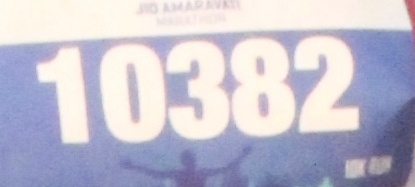
\includegraphics[width=\textwidth]{images/processing/ocr/10382_org}
    \caption{Original Image}
    \label{fig:processing_pipeline:ocr_postprocessing:white_on_dark_original}
  \end{subfigure}
  \hspace{\fill}
  \begin{subfigure}[b]{0.23\textwidth}
    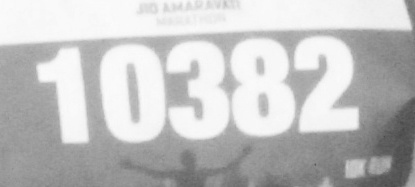
\includegraphics[width=\textwidth]{images/processing/ocr/10382_bw}
    \caption{Greyscale}
  \end{subfigure}
  \hspace{\fill}
  \begin{subfigure}[b]{0.23\textwidth}
    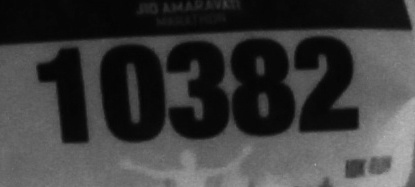
\includegraphics[width=\textwidth]{images/processing/ocr/10382_bw_inv}
    \caption{Inverse Greyscale}
  \end{subfigure}
  \hspace{\fill}
  \begin{subfigure}[b]{0.23\textwidth}
    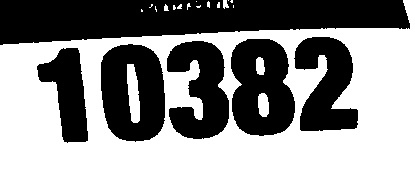
\includegraphics[width=\textwidth]{images/processing/ocr/10382_inv}
    \caption{Binarised}
  \end{subfigure}
  \\ \bigskip
  \hspace{\fill}
  \begin{subfigure}[b]{0.23\textwidth}
    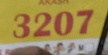
\includegraphics[width=\textwidth]{images/processing/ocr/3207_org}
    \caption{Original Image}
    \label{fig:processing_pipeline:ocr_postprocessing:color_original}
  \end{subfigure}
  \hspace{\fill}
  \begin{subfigure}[b]{0.23\textwidth}
    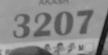
\includegraphics[width=\textwidth]{images/processing/ocr/3207_bw}
    \caption{Greyscale}
  \end{subfigure}
  \hspace{\fill}
  \begin{subfigure}[b]{0.23\textwidth}
    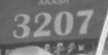
\includegraphics[width=\textwidth]{images/processing/ocr/3207_bw_inv}
    \caption{Inverse Greyscale}
  \end{subfigure}
  \hspace{\fill}
  
  \caption[Image post-processing applied to optimise input into an OCR engine]{Image post-processing applied to optimise input into an \gls{ocr} engine. \textit{Top}: An \gls{rbn} with white numbers can be applied binarised thresholding. \textit{Bottom}: A \gls{rbn} with red numbers cannot have binarised thresholding applied.}
  \label{fig:processing_pipeline:ocr_postprocessing}
\end{figure}

All preprocessed images are provided as input to Tesseract 4 alpha\footnoteurl{https://github.com/tesseract-ocr/tesseract/tree/4.00.00alpha}{5 September 2017}. We use this \gls{ocr} engine as it supports \gls{lstm} \gls{nn}-based character recognition. From all output of our candidates shown in \cref{fig:processing_pipeline:ocr_postprocessing}, multiple text candidates are extracted from Tesseract. To clean our output, we strip out characters that are not within our known character range of A--Z, 0--9 and figure dashes. Additionally, we only accept unique \gls{rbn} sequences per bib region to prevent duplicates.